\documentclass{ltxdoc}

\usepackage{tikz}
\usetikzlibrary{positioning}
\usepackage{pgfmorepages}
\usepackage{fancyvrb}

\GetFileInfo{pgfmorepages.sty}

\title{PGF \emph{more} Pages}
\author{Andrew Stacey \\ \texttt{loopspace@mathforge.org}}
\date{\fileversion\ from \filedate}

\begin{document}

\maketitle

\section{Introduction}

The \Verb+pgfmorepages+ package is a drop-in replacement for the \Verb+pgfpages+ package which comes with TikZ/PGF.
As it is a drop-in replacement, it \emph{ought} to be fully backwards compatible with \Verb+pgfpages+.

\Verb+pgfpages+ allows you the ability to place several pages of your document (hereafter \emph{logical pages}) onto one page of the output (hereafter \emph{physical pages}).
\Verb+pgfmorepages+ adds extra features, the primary one being that whereas \Verb+pgfpages+ is ``many to one'', \Verb+pgfmorepages+ is ``many to many''.
That is, while \Verb+pgfpages+ works one physical page at a time then \Verb+pgfmorepages+ can juggle several logical pages onto several physical pages.

As an example of its capability, the layout \Verb+4 on 2, book format+ places four logical pages onto two physical pages so that when folded it forms a booklet.
The layout is therefore:

\begin{center}
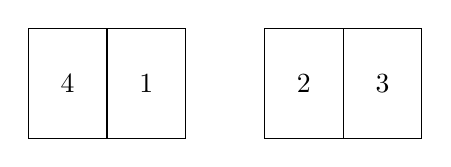
\begin{tikzpicture}
\node at (0,0) {\(4\)};
\node at (1,0) {\(1\)};
\node at (3,0) {\(2\)};
\node at (4,0) {\(3\)};
\draw (-.5,-.7) rectangle (.5,.7);
\draw (1,0)  +(-.5,-.7) rectangle +(.5,.7);
\draw (3,0)  +(-.5,-.7) rectangle +(.5,.7);
\draw (4,0)  +(-.5,-.7) rectangle +(.5,.7);
\end{tikzpicture}
\end{center}

This requires knowing all four logical pages before the first physical page is output.

\section{Usage}

In your preamble:

\begin{verbatim}
\usepackage{pgfmorepages}
\end{verbatim}

\subsection{Layouts}

The original \Verb+pgfpages+ defined the following layouts:

\begin{itemize}
\item \Verb+rounded corners+
\item \Verb+resize to+
\item \Verb+two screens with lagging second+
\item \Verb+two screens with optional second+
\item \Verb+2 on 1+
\item \Verb+4 on 1+
\item \Verb+6 on 1+
\item \Verb+8 on 1+
\item \Verb+16 on 1+
\end{itemize}

The \Verb+pgfmorepages+ defines some extra layouts, which require the following command in your preamble:
%
\begin{verbatim}
\pgfmorepagesloadextralayouts
\end{verbatim}

\begin{itemize}
\item \Verb+4 on 2, odd then even+

\begin{center}
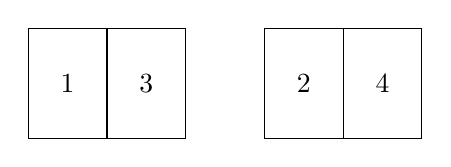
\begin{tikzpicture}
\node at (0,0) {\(1\)};
\node at (1,0) {\(3\)};
\node at (3,0) {\(2\)};
\node at (4,0) {\(4\)};
\draw (-.5,-.7) rectangle (.5,.7);
\draw (1,0)  +(-.5,-.7) rectangle +(.5,.7);
\draw (3,0)  +(-.5,-.7) rectangle +(.5,.7);
\draw (4,0)  +(-.5,-.7) rectangle +(.5,.7);
\end{tikzpicture}
\end{center}

\item \Verb+4 on 2, even then odd+

\begin{center}
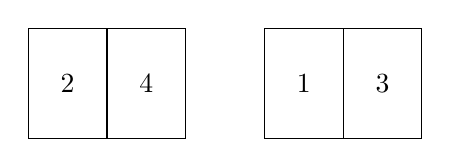
\begin{tikzpicture}
\node at (0,0) {\(2\)};
\node at (1,0) {\(4\)};
\node at (3,0) {\(1\)};
\node at (4,0) {\(3\)};
\draw (-.5,-.7) rectangle (.5,.7);
\draw (1,0)  +(-.5,-.7) rectangle +(.5,.7);
\draw (3,0)  +(-.5,-.7) rectangle +(.5,.7);
\draw (4,0)  +(-.5,-.7) rectangle +(.5,.7);
\end{tikzpicture}
\end{center}

\item \Verb+4 on 2, book format+

\begin{center}
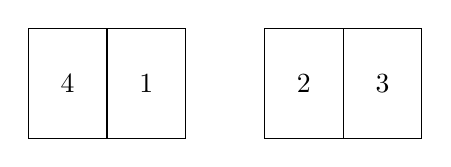
\begin{tikzpicture}
\node at (0,0) {\(4\)};
\node at (1,0) {\(1\)};
\node at (3,0) {\(2\)};
\node at (4,0) {\(3\)};
\draw (-.5,-.7) rectangle (.5,.7);
\draw (1,0)  +(-.5,-.7) rectangle +(.5,.7);
\draw (3,0)  +(-.5,-.7) rectangle +(.5,.7);
\draw (4,0)  +(-.5,-.7) rectangle +(.5,.7);
\end{tikzpicture}
\end{center}

\item \Verb+8 on 4, book format+

\begin{center}
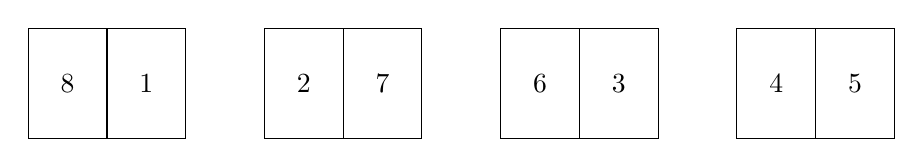
\begin{tikzpicture}
\node at (0,0) {\(8\)};
\node at (1,0) {\(1\)};
\node at (3,0) {\(2\)};
\node at (4,0) {\(7\)};
\node at (6,0) {\(6\)};
\node at (7,0) {\(3\)};
\node at (9,0) {\(4\)};
\node at (10,0) {\(5\)};
\draw (-.5,-.7) rectangle (.5,.7);
\draw (1,0)  +(-.5,-.7) rectangle +(.5,.7);
\draw (3,0)  +(-.5,-.7) rectangle +(.5,.7);
\draw (4,0)  +(-.5,-.7) rectangle +(.5,.7);
\draw (6,0)  +(-.5,-.7) rectangle +(.5,.7);
\draw (7,0)  +(-.5,-.7) rectangle +(.5,.7);
\draw (9,0)  +(-.5,-.7) rectangle +(.5,.7);
\draw (10,0)  +(-.5,-.7) rectangle +(.5,.7);
\end{tikzpicture}
\end{center}

\item \Verb+8 on 4, book format, reverse second, single sided+

\begin{center}
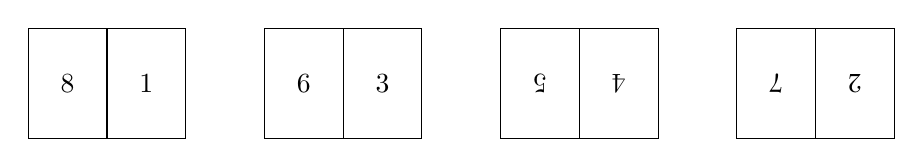
\begin{tikzpicture}
\node at (0,0) {\(8\)};
\node at (1,0) {\(1\)};
\node at (3,0) {\(6\)};
\node at (4,0) {\(3\)};
\node[rotate=180] at (6,0) {\(5\)};
\node[rotate=180] at (7,0) {\(4\)};
\node[rotate=180] at (9,0) {\(7\)};
\node[rotate=180] at (10,0) {\(2\)};
\draw (-.5,-.7) rectangle (.5,.7);
\draw (1,0)  +(-.5,-.7) rectangle +(.5,.7);
\draw (3,0)  +(-.5,-.7) rectangle +(.5,.7);
\draw (4,0)  +(-.5,-.7) rectangle +(.5,.7);
\draw (6,0)  +(-.5,-.7) rectangle +(.5,.7);
\draw (7,0)  +(-.5,-.7) rectangle +(.5,.7);
\draw (9,0)  +(-.5,-.7) rectangle +(.5,.7);
\draw (10,0)  +(-.5,-.7) rectangle +(.5,.7);
\end{tikzpicture}
\end{center}


\item \Verb+5 index cards+
\item \Verb+repeated 2-up+

\begin{center}
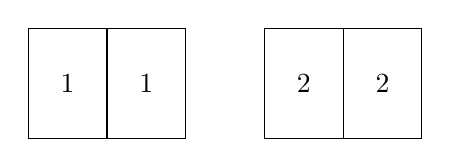
\begin{tikzpicture}
\node at (0,0) {\(1\)};
\node at (1,0) {\(1\)};
\node at (3,0) {\(2\)};
\node at (4,0) {\(2\)};
\draw (-.5,-.7) rectangle (.5,.7);
\draw (1,0)  +(-.5,-.7) rectangle +(.5,.7);
\draw (3,0)  +(-.5,-.7) rectangle +(.5,.7);
\draw (4,0)  +(-.5,-.7) rectangle +(.5,.7);
\end{tikzpicture}
\end{center}

\item \Verb+repeated 4-up+

\begin{center}
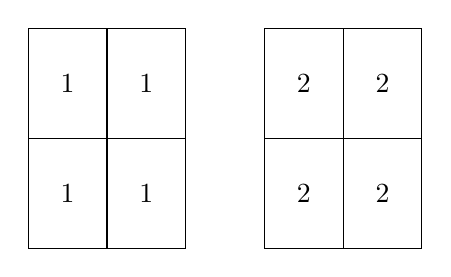
\begin{tikzpicture}
\node at (0,0) {\(1\)};
\node at (1,0) {\(1\)};
\node at (0,1.4) {\(1\)};
\node at (1,1.4) {\(1\)};
\node at (3,0) {\(2\)};
\node at (4,0) {\(2\)};
\node at (3,1.4) {\(2\)};
\node at (4,1.4) {\(2\)};
\draw (-.5,-.7) rectangle (.5,.7);
\draw (1,0)  +(-.5,-.7) rectangle +(.5,.7);
\draw (3,0)  +(-.5,-.7) rectangle +(.5,.7);
\draw (4,0)  +(-.5,-.7) rectangle +(.5,.7);
\draw (0,1.4)  +(-.5,-.7) rectangle +(.5,.7);
\draw (1,1.4)  +(-.5,-.7) rectangle +(.5,.7);
\draw (3,1.4)  +(-.5,-.7) rectangle +(.5,.7);
\draw (4,1.4)  +(-.5,-.7) rectangle +(.5,.7);
\end{tikzpicture}
\end{center}


\item \Verb+1 on 1+

This is a layout that ``resets'' the mechanism back to one logical page on one physical page.
It still uses the mechanics of the \Verb+pgfmorepages+ package so is not quite the same as removing it altogether, but is effectively the same.

\item \Verb+discard+

This layout discards all its pages.
Useful to remove pages from a document without changing the source file too much.

\end{itemize}

To use a layout, use the command:
%
\begin{verbatim}
\pgfpagesuselayout{<layout name>}[<optional arguments>]
\end{verbatim}



\subsection{Options}

The optional arguments are a superset of the ones that \Verb+pgfpages+ allows.

\begin{itemize}
\item \Verb+physical paper width+
\item \Verb+physical paper height+
\item \Verb+a0paper+
\item \Verb+a1paper+
\item \Verb+a2paper+
\item \Verb+a3paper+
\item \Verb+a4paper+
\item \Verb+a5paper+
\item \Verb+a6paper+
\item \Verb+letterpaper+
\item \Verb+legalpaper+
\item \Verb+executivepaper+
\item \Verb+landscape+
\item \Verb+border shrink+
\item \Verb+border code+
\item \Verb+corner width+
\item \Verb+odd numbered pages right+
\item \Verb+second right+
\item \Verb+second left+
\item \Verb+second top+
\item \Verb+second bottom+
\end{itemize}

The only additional option is \Verb+border code+ which, if the layout does anything with it, is designed for passing a command to the layout for the border path.
The intention of this is that sometimes it is useful to draw the page border when designing a document but you might want to disable it for the final version.
This makes it easy to switch between those (providing the layout supports it).

\subsection{Changing Layout}

The documentation for \Verb+pgfpages+ states that it is possible to change layout mid-document.
This turns out not to be correct for \Verb+pgfpages+ as it doesn't reset everything correctly.
\Verb+pgfmorepages+ fixes this\footnote{Or tries to -- I keep discovering new options that I haven't reset properly.}.
It is best practice to use a \Verb+\newpage+ or \Verb+\clearpage+ before doing so.
The layout \Verb+1 on 1+ is useful here as it sets the layout back to one logical page on one physical page.

\section{Defining a New Layout}

The best way to define a new layout is to start with one of the predefined ones and modify it.
To that end, here is an example layout with comments.

\begin{verbatim}
 % Set the name of the layout
\pgfpagesdeclarelayout{4 on 2, book format}% 
{%
 % Unless overridden, this layout uses the same paper size
 % but rotated so that two logical pages fit naturally on
 % one physical page
  \edef\pgfpageoptionheight{\the\paperwidth}
  \edef\pgfpageoptionwidth{\the\paperheight}
 % Defaults for the border
  \def\pgfpageoptionborder{0pt}
  \def\pgfpageoptionbordercode{}
 % Start with the first page of the document
  \def\pgfpageoptionfirstshipout{1}
}%
{%
 % These are the settings for the physical pages
  \pgfpagesphysicalpageoptions
  {%
 % Each set consists of 4 logical and 2 physical pages
    logical pages=4,%
    physical pages=2,%
    physical height=\pgfpageoptionheight,%
    physical width=\pgfpageoptionwidth,%
    current logical shipout=\pgfpageoptionfirstshipout%
  }
 % These are the settings for the logical pages.
 % These hold for all the logical pages.
  \pgfpagessetdefaults{%
    border code=\pgfpageoptionbordercode
  }
 % Our arrangement is different for two portrait pages
 % on one landscape as opposed to two landscape on
 % one portrait.
 % This is for two portrait on one landscape
  \ifdim\paperheight>\paperwidth\relax
    % put side-by-side
 % There are several ways to declare which logical page
 % goes on which physical page.  This command sets the
 % physical page for the following logical pages.  The
 % second argument is any options to be set for that
 % physical page. 
  \pgfpagesphysicalpage{1}{}
 % Our fourth logical page goes on the first physical page
    \pgfpageslogicalpageoptions{4}
    {%
      border shrink=\pgfpageoptionborder,%
      resized width=.5\pgfphysicalwidth,%
      resized height=\pgfphysicalheight,%
      center=\pgfpoint{.25\pgfphysicalwidth}{.5\pgfphysicalheight}%
    }%
 % The second and third logical pages go on the second
 % physical page.
  \pgfpagesphysicalpage{2}{}
    \pgfpageslogicalpageoptions{3}
    {%
      border shrink=\pgfpageoptionborder,%
      resized width=.5\pgfphysicalwidth,%
      resized height=\pgfphysicalheight,%
      center=\pgfpoint{.75\pgfphysicalwidth}{.5\pgfphysicalheight}%
    }%
    \pgfpageslogicalpageoptions{2}
    {%
      border shrink=\pgfpageoptionborder,%
      resized width=.5\pgfphysicalwidth,%
      resized height=\pgfphysicalheight,%
      center=\pgfpoint{.25\pgfphysicalwidth}{.5\pgfphysicalheight}%
    }%
 % The first logical page goes back on the first physical page.
  \pgfpagesphysicalpage{1}{}
    \pgfpageslogicalpageoptions{1}
    {%
      border shrink=\pgfpageoptionborder,%
      resized width=.5\pgfphysicalwidth,%
      resized height=\pgfphysicalheight,%
      center=\pgfpoint{.75\pgfphysicalwidth}{.5\pgfphysicalheight}%
    }%
  \else
 % These are essentially the same as above, except with
 % two landscape pages on one portrait, so the pages
 % are in different locations.
    % stack on top of one another
  \pgfpagesphysicalpage{1}{}
    \pgfpageslogicalpageoptions{4}
    {%
      border shrink=\pgfpageoptionborder,%
      resized width=\pgfphysicalwidth,%
      resized height=.5\pgfphysicalheight,%
      center=\pgfpoint{.5\pgfphysicalwidth}{.75\pgfphysicalheight}%
    }%
  \pgfpagesphysicalpage{2}{}
    \pgfpageslogicalpageoptions{3}
    {%
      border shrink=\pgfpageoptionborder,%
      resized width=\pgfphysicalwidth,%
      resized height=.5\pgfphysicalheight,%
      center=\pgfpoint{.5\pgfphysicalwidth}{.25\pgfphysicalheight}%
    }%
    \pgfpageslogicalpageoptions{2}
    {%
      border shrink=\pgfpageoptionborder,%
      resized width=\pgfphysicalwidth,%
      resized height=.5\pgfphysicalheight,%
      center=\pgfpoint{.5\pgfphysicalwidth}{.75\pgfphysicalheight}%
    }%
  \pgfpagesphysicalpage{2}{}
    \pgfpageslogicalpageoptions{1}
    {%
      border shrink=\pgfpageoptionborder,%
      resized width=\pgfphysicalwidth,%
      resized height=.5\pgfphysicalheight,%
      center=\pgfpoint{.5\pgfphysicalwidth}{.25\pgfphysicalheight}%
    }%
  \fi    
}
\end{verbatim}

\end{document}
